% Bổ sung vào Chương 2 - sau phần lý thuyết BERT
\newpage
\subsection{Công nghệ nền tảng và framework}

\subsubsection{Python và hệ sinh thái Deep Learning}

\subsubsubsection{Python trong phân tích dữ liệu và AI}

Python đã trở thành ngôn ngữ lập trình tiêu chuẩn cho các ứng dụng Machine Learning và Deep Learning nhờ tính đơn giản, dễ học và hệ sinh thái thư viện phong phú. Đối với bài toán dự báo giao thông, Python cung cấp đầy đủ công cụ từ xử lý dữ liệu, huấn luyện mô hình đến triển khai sản phẩm.

Các ưu điểm chính bao gồm cú pháp rõ ràng giúp code dễ đọc và bảo trì, thư viện phong phú như NumPy, Pandas, Scikit-learn, PyTorch, TensorFlow, Transformers, cộng đồng lớn hỗ trợ tốt, và khả năng tích hợp với nhiều hệ thống và database khác nhau.

\subsubsubsection{PyTorch}

\textbf{PyTorch Core}

PyTorch là framework deep learning được phát triển bởi Meta AI, nổi bật với cơ chế dynamic computational graph cho phép debug và thử nghiệm linh hoạt. PyTorch cung cấp các thành phần cốt lõi như tensor operations với hỗ trợ GPU, module system để xây dựng mạng neural network, các thuật toán tối ưu (AdamW, SGD, RMSprop), và cơ chế automatic differentiation cho backpropagation.

Kiến trúc của PyTorch được thiết kế theo nguyên tắc modular, cho phép research scientists dễ dàng thử nghiệm các ý tưởng mới trong khi vẫn đảm bảo hiệu năng cao khi triển khai production.

\subsubsection{Kiến trúc Kappa cho xử lý dữ liệu streaming}

\subsubsubsection{Tổng quan về Kappa Architecture}

Kiến trúc Kappa là một mô hình xử lý dữ liệu hiện đại được đề xuất bởi Jay Kreps (LinkedIn) như một giải pháp đơn giản hóa so với Lambda Architecture truyền thống. Khác với Lambda Architecture có hai đường xử lý riêng biệt (batch và stream), Kappa Architecture chỉ sử dụng một đường xử lý streaming duy nhất, giảm độ phức tạp và chi phí bảo trì.

\begin{figure}[h]
    \centering
    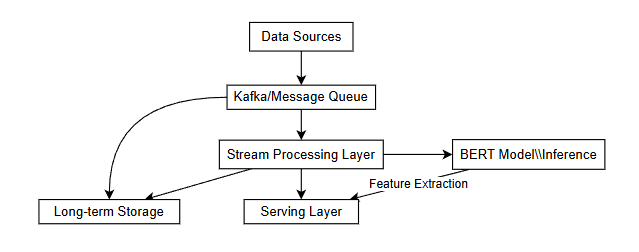
\includegraphics[width=1\textwidth]{Images/kappa_bert_architecture.png}
    \caption{Kiến trúc Kappa với BERT Model Integration}
    \label{fig:kappa_bert}
\end{figure}


\textbf{Các thành phần chính:}

\begin{enumerate}
    \item \textbf{Message Queue (Kafka)}: Nhận và lưu trữ tất cả dữ liệu đầu vào dưới dạng event log bất biến. Kafka đóng vai trò là single source of truth, cho phép replay dữ liệu khi cần thiết.
    
    \item \textbf{Stream Processing Layer}: Xử lý dữ liệu theo thời gian thực, thực hiện transformations, aggregations, và feature engineering cho BERT model.
    
    \item \textbf{ML Model Inference}: BERT model được deploy để thực hiện prediction trên streaming data.
    
    \item \textbf{Serving Layer}: Lưu trữ kết quả prediction và phục vụ các truy vấn từ applications.
    
    \item \textbf{Long-term Storage}: Lưu trữ dữ liệu lịch sử cho mục đích retraining model và analysis.
\end{enumerate}

\subsubsubsection{Apache Kafka làm backbone}

Apache Kafka là distributed streaming platform đóng vai trò trung tâm trong Kappa Architecture. Kafka được thiết kế như một commit log phân tán, nơi mọi message được lưu trữ theo thứ tự và có thể được đọc lại nhiều lần.

\textbf{Các khái niệm cốt lõi:}

\begin{itemize}
    \item \textbf{Topics}: Danh mục logic để phân loại messages. Ví dụ: traffic\_speed, traffic\_volume, traffic\_incidents.
    
    \item \textbf{Partitions}: Mỗi topic được chia thành nhiều partitions để tăng khả năng song song hóa và throughput.
    
    \item \textbf{Producers}: Các services ghi dữ liệu vào Kafka topics.
    
    \item \textbf{Consumers}: Các services đọc và xử lý dữ liệu từ topics.
    
    \item \textbf{Consumer Groups}: Nhóm consumers làm việc cùng nhau để xử lý song song dữ liệu từ một topic.
\end{itemize}

\textbf{Ưu điểm của Kafka trong hệ thống giao thông:}

\begin{itemize}
    \item \textbf{High Throughput}: Xử lý hàng triệu messages/giây từ các cảm biến giao thông
    \item \textbf{Durability}: Messages được replicate và persist, đảm bảo không mất dữ liệu
    \item \textbf{Scalability}: Dễ dàng scale horizontal bằng cách thêm brokers và partitions
    \item \textbf{Replay Capability}: Có thể đọc lại dữ liệu lịch sử để recompute hoặc fix bugs
    \item \textbf{Low Latency}: Độ trễ chỉ vài milliseconds, phù hợp cho real-time applications
\end{itemize}

\subsubsubsection{So sánh Kappa với Lambda Architecture}

\begin{table}[h]
\centering
\caption{So sánh Kappa và Lambda Architecture}
\begin{tabular}{|p{3.5cm}|p{5cm}|p{5cm}|}
\hline
\textbf{Tiêu chí} & \textbf{Lambda Architecture} & \textbf{Kappa Architecture} \\ \hline
Batch Layer & Có (MapReduce/Spark) & Không có \\ \hline
Speed Layer & Có (Stream Processing) & Stream processing duy nhất \\ \hline
Độ phức tạp & Cao (2 codebases riêng) & Thấp (1 codebase) \\ \hline
Độ trễ & Cao hơn do batch & Thấp, real-time \\ \hline
Consistency & Eventual consistency & Easier to maintain \\ \hline
Reprocessing & Cần chạy lại batch job & Replay từ Kafka \\ \hline
Maintenance & Khó (sync 2 systems) & Dễ hơn \\ \hline
Use case phù hợp & Cần cả batch và stream & Streaming-first applications \\ \hline
\end{tabular}
\label{tab:kappa_lambda}
\end{table}

\subsubsubsection{Ứng dụng Kappa trong hệ thống giao thông}

Trong bài toán phân tích giao thông, Kappa Architecture phù hợp vì:

\begin{enumerate}
    \item \textbf{Tính real-time}: Dữ liệu giao thông cần được xử lý ngay lập tức để cảnh báo kịp thời.
    
    \item \textbf{Data replay}: Khi cần retrain model hoặc fix bugs, có thể replay dữ liệu từ Kafka mà không cần maintain batch pipeline riêng.
    
    \item \textbf{Unified logic}: Cùng một đoạn code xử lý được sử dụng cho cả real-time và historical analysis.
    
    \item \textbf{Event-driven}: Giao thông là event-driven system (xe đi qua cảm biến, tắc nghẽn xảy ra, tai nạn), phù hợp với stream processing.
\end{enumerate}

\textbf{Pipeline xử lý trong hệ thống:}

\begin{enumerate}
    \item Cảm biến giao thông (camera, loop detectors, GPS) publish data vào Kafka topics
    \item Consumers đọc từ Kafka, thực hiện:
    \begin{itemize}
        \item Data cleaning và validation
        \item Feature extraction (tốc độ, volume, occupancy)
        \item Windowed aggregations (5-min, 15-min averages)
        \item Anomaly detection
        \item Correlation analysis
    \end{itemize}
    \item Kết quả được ghi vào:
    \begin{itemize}
        \item \textbf{Apache Parquet} (định dạng lưu trữ cột cho phân tích dữ liệu quy mô lớn)
    \end{itemize}
    \item ML models subscribe processed data để thực hiện predictions
    \item Results được publish lại vào Kafka để downstream services consume
\end{enumerate}
\subsubsection{TomTom Historical Traffic Stats API}

TomTom cung cấp dữ liệu giao thông lịch sử với độ bao phủ cao, bao gồm tốc độ trung bình, mức độ tắc nghẽn và chỉ số độ trễ theo từng đoạn đường. Dữ liệu được tổng hợp từ nhiều nguồn GPS và cập nhật theo khoảng thời gian từ 1--5 phút.

\paragraph{Ưu điểm}
\begin{itemize}
    \item Dữ liệu lịch sử dài hạn, hỗ trợ phân tích xu hướng theo giờ, ngày và tuần.
    \item Độ bao phủ rộng giúp bù đắp cho các khu vực thiếu cảm biến tại địa phương.
    \item Dễ dàng tích hợp vào các mô hình học chuỗi thời gian và mô hình mạng lưới.
\end{itemize}

\paragraph{Hạn chế}
\begin{itemize}
    \item Không phản ánh nguyên nhân của tắc nghẽn, chỉ mô tả hiện tượng.
    \item Chi phí sử dụng có thể cao nếu mở rộng cho toàn thành phố.
\end{itemize}

\paragraph{Vai trò trong đề tài}
Dữ liệu lịch sử từ TomTom giúp:
\begin{itemize}
    \item Huấn luyện mô hình dự báo giao thông.
    \item Phân tích lan truyền tắc nghẽn giữa các đoạn đường.
    \item Xây dựng dữ liệu đầu vào cho mô hình học sâu theo dạng đồ thị.
\end{itemize}

\subsubsection{Cơ sở dữ liệu và lưu trữ}

\subsubsubsection{Lưu trữ dữ liệu dạng cột với Apache Parquet}

Trong hệ thống phân tích giao thông đô thị, dữ liệu đầu vào có đặc trưng khối lượng lớn, cấu trúc rõ ràng và chủ yếu phục vụ cho các tác vụ phân tích, thống kê và huấn luyện mô hình học máy. Do đó, hệ thống lựa chọn \textbf{Apache Parquet} làm định dạng lưu trữ chính thay vì cơ sở dữ liệu giao dịch truyền thống.

Parquet là định dạng lưu trữ dạng cột (columnar storage), được thiết kế tối ưu cho các hệ thống phân tích dữ liệu lớn (Big Data Analytics) và các workload đọc nhiều, ghi ít.

\textbf{Các đặc điểm kỹ thuật chính của Parquet:}

\begin{itemize}
    \item \textbf{Columnar Storage}: Dữ liệu được lưu theo cột thay vì theo hàng, giúp giảm lượng dữ liệu cần đọc khi chỉ truy vấn một số thuộc tính cụ thể (ví dụ: tốc độ, lưu lượng, thời gian).
    
    \item \textbf{Efficient Compression}: Parquet hỗ trợ nhiều thuật toán nén (Snappy, ZSTD, GZIP), tận dụng tính đồng nhất của dữ liệu trong cùng một cột để đạt tỷ lệ nén cao, giảm đáng kể dung lượng lưu trữ.
    
    \item \textbf{Predicate Pushdown}: Cho phép loại bỏ sớm các block dữ liệu không thỏa điều kiện truy vấn, giúp tăng tốc độ xử lý.
    
    \item \textbf{Schema Evolution}: Hỗ trợ thay đổi schema theo thời gian (thêm/bớt cột) mà không làm hỏng dữ liệu cũ, phù hợp với dữ liệu giao thông có thể mở rộng thuộc tính.
    
    \item \textbf{Cross-platform Compatibility}: Tương thích tốt với các hệ sinh thái phân tích như Apache Spark, Pandas, DuckDB và các thư viện học máy.
\end{itemize}



\subsubsubsection{Ứng dụng Parquet trong hệ thống giao thông}

Trong hệ thống đề xuất, Parquet được sử dụng để lưu trữ các tập dữ liệu giao thông đã qua xử lý (processed data), bao gồm:

\begin{itemize}
    \item Thông tin các đoạn đường (road segments)
    \item Đặc trưng giao thông theo thời gian (speed, volume, congestion level)
    \item Dữ liệu đặc trưng đầu vào cho mô hình học máy
    \item Kết quả dự đoán và thống kê theo từng khung thời gian
\end{itemize}

Dữ liệu được tổ chức theo cấu trúc thư mục phân tầng dựa trên thời gian (theo ngày, giờ hoặc batch xử lý), giúp thuận tiện cho việc truy xuất, huấn luyện mô hình và phân tích hậu kỳ.
\subsubsection{API và Web Development Stack}

\subsubsubsection{FastAPI}

FastAPI là một web framework hiện đại dành cho Python, được thiết kế để xây dựng các dịch vụ API với hiệu năng cao, cú pháp rõ ràng và khả năng mở rộng tốt. Framework này đặc biệt phù hợp cho các hệ thống xử lý dữ liệu và mô hình học máy nhờ khả năng tích hợp chặt chẽ với hệ sinh thái Python.

\textbf{Các đặc điểm kỹ thuật chính của FastAPI:}

\begin{itemize}
    \item \textbf{High Performance}: FastAPI được xây dựng trên nền Starlette và Pydantic, cho hiệu năng xử lý cao, đáp ứng tốt các yêu cầu API có tần suất truy cập lớn.
    
    \item \textbf{Type-based Validation}: Sử dụng Python type hints để tự động kiểm tra, xác thực và chuyển đổi dữ liệu đầu vào, giúp giảm lỗi và tăng độ tin cậy của hệ thống.
    
    \item \textbf{Asynchronous Processing}: Hỗ trợ native \texttt{async/await}, cho phép xử lý đồng thời nhiều request, phù hợp với các pipeline phân tích dữ liệu và inference mô hình.
    
    \item \textbf{Automatic API Documentation}: Tự động sinh tài liệu OpenAPI (Swagger) và ReDoc, giúp việc kiểm thử và tích hợp API trở nên thuận tiện.
    
    \item \textbf{Modular Architecture}: Dễ dàng tổ chức code theo các module (router, service, schema), phù hợp cho các hệ thống nghiên cứu và phát triển mở rộng.
\end{itemize}

Trong hệ thống giao thông được đề xuất, FastAPI đóng vai trò là lớp trung gian cung cấp các API phục vụ:
\begin{itemize}
    \item Truy xuất dữ liệu giao thông đã được xử lý và lưu trữ dưới dạng Parquet
    \item Cung cấp đầu vào và đầu ra cho mô hình học máy
    \item Kết nối giữa pipeline xử lý dữ liệu và giao diện trực quan
\end{itemize}

\subsubsubsection{Streamlit}

Streamlit là framework Python nhẹ, được thiết kế để xây dựng nhanh các ứng dụng web phục vụ trực quan hóa dữ liệu và trình diễn kết quả phân tích mà không cần phát triển frontend phức tạp.

\textbf{Ưu điểm của Streamlit trong bối cảnh nghiên cứu và đồ án:}

\begin{itemize}
    \item \textbf{Rapid Prototyping}: Cho phép xây dựng giao diện trực quan chỉ với một lượng nhỏ mã Python, rút ngắn thời gian phát triển.
    
    \item \textbf{Tight Integration with Data Stack}: Tích hợp trực tiếp với Pandas, NumPy, PyArrow và các thư viện học máy, phù hợp cho việc hiển thị dữ liệu Parquet và kết quả mô hình.
    
    \item \textbf{Interactive Visualization}: Hỗ trợ tương tác người dùng theo thời gian thực (filter, slider, selection) cho các phân tích giao thông.
    
    \item \textbf{Lightweight Deployment}: Không yêu cầu quản lý state phức tạp hay frontend build system, phù hợp cho môi trường nghiên cứu và demo hệ thống.
\end{itemize}

Trong hệ thống này, Streamlit được sử dụng để:
\begin{itemize}
    \item Trực quan hóa dữ liệu giao thông theo không gian và thời gian
    \item Hiển thị kết quả dự đoán và phân tích của mô hình
    \item Phục vụ mục đích demo, đánh giá và trình bày hệ thống
\end{itemize}

Cách tiếp cận kết hợp FastAPI và Streamlit giúp tách biệt rõ ràng giữa lớp xử lý nghiệp vụ và lớp trình diễn, đảm bảo tính đơn giản, dễ bảo trì và phù hợp với mục tiêu nghiên cứu của đề tài.

\subsubsection{Containerization và Orchestration}

\subsubsubsection{Docker}

Docker là platform containerization cho phép đóng gói applications và dependencies thành containers độc lập, nhất quán trên mọi môi trường từ development đến production.

\textbf{Lợi ích của Docker:}

\begin{itemize}
    \item \textbf{Consistency}: "Works on my machine" problem được giải quyết
    \item \textbf{Isolation}: Mỗi service chạy trong môi trường riêng
    \item \textbf{Portability}: Deploy trên bất kỳ platform nào hỗ trợ Docker
    \item \textbf{Resource Efficiency}: Lightweight hơn VMs, chia sẻ kernel
    \item \textbf{Versioning}: Image versioning cho rollback dễ dàng
\end{itemize}

\textbf{Docker Compose} quản lý multi-container applications, định nghĩa toàn bộ stack (API, databases, cache, message queue) trong một file YAML, cho phép start/stop toàn bộ hệ thống với một command.

\subsubsubsection{Kubernetes}

Kubernetes (K8s) là container orchestration platform mã nguồn mở, tự động hóa việc deploy, scale, và manage containerized applications trong môi trường production.

\textbf{Khái niệm cốt lõi:}

\begin{itemize}
    \item \textbf{Pods}: Đơn vị nhỏ nhất, chứa một hoặc nhiều containers
    \item \textbf{ReplicaSets}: Đảm bảo số lượng pod replicas mong muốn
    \item \textbf{Deployments}: Quản lý rolling updates và rollbacks
    \item \textbf{Services}: Expose pods qua stable network endpoint
    \item \textbf{Ingress}: HTTP routing và load balancing
    \item \textbf{ConfigMaps và Secrets}: Quản lý configuration và sensitive data
    \item \textbf{Persistent Volumes}: Storage abstraction cho stateful apps
    \item \textbf{Namespaces}: Logical isolation giữa các môi trường
\end{itemize}

\textbf{Tính năng quan trọng cho production:}

\begin{enumerate}
    \item \textbf{Auto-scaling}: Horizontal Pod Autoscaler (HPA) tự động scale dựa trên CPU, memory, hoặc custom metrics
    
    \item \textbf{Self-healing}: Tự động restart failed containers, replace và reschedule pods khi nodes die
    
    \item \textbf{Service Discovery và Load Balancing}: Tự động distribute traffic đến healthy pods
    
    \item \textbf{Rolling Updates}: Zero-downtime deployments với progressive rollout
    
    \item \textbf{Resource Management}: CPU và memory requests/limits để optimize cluster utilization
\end{enumerate}

Với hệ thống giao thông cần high availability và khả năng scale dynamic theo traffic load, Kubernetes cung cấp infrastructure layer mạnh mẽ để đảm bảo reliability và performance.

\subsection{Tóm tắt stack công nghệ}

Bảng dưới đây tóm tắt các công nghệ chính được sử dụng trong đề tài:

\begin{table}[h]
\centering
\caption{Stack công nghệ hệ thống}
\begin{tabular}{|l|l|l|}
\hline
\textbf{Layer} & \textbf{Technology} & \textbf{Purpose} \\ \hline
Programming & Python 3.11+ & Main development language \\ \hline
ML Framework & PyTorch 2.0+ & Deep learning models \\ \hline
Graph Library & PyTorch Geometric & GNN implementation \\ \hline
Message Queue & Apache Kafka & Event streaming backbone \\ \hline
Stream Processing & Python + Kafka & Real-time data processing \\ \hline
Storage & Apache Parquet & Long-term historical data \\ \hline
% Cache & Redis & In-memory data store \\ \hline
Model Serving & FastAPI + PyTorch & Inference API \\ \hline
% Monitoring & Prometheus + Grafana & Metrics và visualization \\ \hline
\end{tabular}
\label{tab:tech_stack}
\end{table}

Kiến trúc này được thiết kế để:
\begin{itemize}
    \item Xử lý dữ liệu streaming real-time hiệu quả
    \item Scale horizontal khi traffic tăng
    \item Maintain low latency cho inference
    \item Support reprocessing và retraining
    \item Provide observability và monitoring đầy đủ
\end{itemize}


\newpage
\subsection{Kết chương}

Chương 2 đã trình bày một cách toàn diện nền tảng lý thuyết và công nghệ cần thiết để xây dựng hệ thống phân tích mối liên hệ giao thông đô thị. Những kiến thức này tạo thành bộ công cụ quan trọng phục vụ cho các chương tiếp theo của đồ án.

\textbf{Về mặt lý thuyết}, chúng ta đã nắm được:

\begin{itemize}
    \item Đặc điểm phức tạp của giao thông đô thị TP.HCM với cơ cấu phương tiện đặc thù, tỷ lệ xe máy chiếm ưu thế tuyệt đối (>90\%), và hiện tượng lan truyền tắc nghẽn theo mạng lưới đường. Việc hiểu rõ bản chất này giúp thiết kế mô hình phù hợp với đặc thù địa phương.

    \item Cơ sở toán học vững chắc về biểu diễn mạng giao thông dưới dạng đồ thị $\mathcal{G} = (\mathcal{V}, \mathcal{E}, \mathcal{A})$, các phép biến đổi trên cấu trúc đồ thị, và cách mô hình hóa tương quan không gian-thời gian.   

    \item Các kiến trúc Graph Neural Networks tiên tiến như GCN và GAT, cho phép học các mối quan hệ phức tạp giữa các nút giao thông mà không cần định nghĩa thủ công. Cơ chế message passing và attention mechanism là nền tảng để mô hình tự động phát hiện các mối tương quan ẩn.

    \item Các mô hình chuỗi thời gian từ RNN cơ bản đến LSTM và GRU, giúp nắm bắt phụ thuộc temporal với khả năng học long-term dependencies. Việc hiểu rõ ưu nhược điểm của từng loại giúp lựa chọn kiến trúc phù hợp cho bài toán dự báo đa bước (multi-step prediction).
\end{itemize}

\textbf{Về mặt công nghệ}, chương này đã xác định được bộ khung kỹ thuật (Technology Stack) hiện đại và mạnh mẽ để hiện thực hóa hệ thống:

\begin{itemize}
    \item \textbf{Hệ sinh thái Python \& PyTorch}: Cung cấp môi trường phát triển linh hoạt, đặc biệt là thư viện PyTorch Geometric chuyên dụng cho các mô hình GNN, giúp đơn giản hóa việc cài đặt các thuật toán phức tạp trên dữ liệu đồ thị.
    
    \item \textbf{Kiến trúc Kappa \& Apache Kafka}: Đảm bảo khả năng xử lý dữ liệu streaming thời gian thực với độ trễ thấp và độ tin cậy cao, phù hợp với đặc thù dữ liệu liên tục từ các cảm biến giao thông.
    
    \item \textbf{Lưu trữ dữ liệu không gian -- thời gian}: Hệ thống sử dụng định dạng Apache Parquet để lưu trữ dữ liệu giao thông có đặc trưng vừa mang thông tin không gian (tọa độ, đoạn đường), vừa mang tính chuỗi thời gian. Cách tiếp cận này cho phép tổ chức dữ liệu theo các phân vùng thời gian và thuộc tính không gian, đồng thời tối ưu hiệu năng cho các tác vụ phân tích, thống kê và huấn luyện mô hình học máy.
    
    \item \textbf{Hạ tầng triển khai}: Việc sử dụng Docker và Kubernetes đảm bảo hệ thống có khả năng mở rộng (scalability), dễ dàng triển khai và vận hành ổn định trong môi trường thực tế.
\end{itemize}

Sự kết hợp chặt chẽ giữa các nền tảng lý thuyết vững chắc và các công nghệ tiên tiến này là tiền đề quan trọng để bước sang Chương 3 -- nơi chúng ta sẽ khảo sát các công trình liên quan để định vị rõ hơn đóng góp của đề tài, và Chương 4 -- nơi mô hình hệ thống cụ thể sẽ được đề xuất.